\documentclass[11pt]{scrartcl}
\usepackage{geometry}                % See geometry.pdf to learn the layout options. There are lots.
\geometry{letterpaper}                   % ... or a4paper or a5paper or ... 
%\geometry{landscape}                % Activate for for rotated page geometry
%\usepackage[parfill]{parskip}    % Activate to begin paragraphs with an empty line rather than an indent
\usepackage{graphicx}
\usepackage{amssymb}
\usepackage{epstopdf}
\DeclareGraphicsRule{.tif}{png}{.png}{`convert #1 `dirname #1`/`basename #1 .tif`.png}

\usepackage{algorithm}
\usepackage{algpseudocode}
%\usepackage{subfig}
%\usepackage{caption}
\usepackage{amsmath}

\usepackage{subcaption}

\title{EM and Three Dimensional Block Modeling\\in Cognitive Social Structures}
\author{Alexander Loewi}
%\date{}                                           % Activate to display a given date or no date

\begin{document}
\maketitle
%\section{}
%\subsection{}

Evidence continues to accumulate that two people in the same social network can have radically different perceptions of that network. They disagree on who is more central, who is friends with whom, and even whether they have a relationship themselves. Whether this comes as a deep surprise or sounds like the most obvious thing in the world, this insight has generated an enormous amount of interest over the last three decades.

While there is no question that the findings are qualitatively compelling, there is also no question that the data that represents them is quantitatively difficult. While many techniques have been developed for operating on single social networks, there are far fewer techniques for dealing with several networks at once, and in particular the multiple networks that represent different perceptions. In addition, those few techniques that have been developed tend to suffer from two serious problems. First, they tend not to be well integrated into familiar statistical frameworks, meaning their theoretical properties are often still in question. Second, they often operate by forcing the multiple networks into a single network, potentially losing all of the structure that makes the differences interesting.

This paper takes two extremely well established statistical methods -- Expectation Maximization and Stochastic Block Models -- and uses them to perform a number of important tasks on the totality of Cognitive Social Structure (network perception) data. Broadly, these tasks fall into the categories of edge inference, and group discovery, although both of these characterizations have some nuance to them. The methods developed here allow for a principled approach to missing data -- an almost universal problem, when trying to collect network perceptions -- as well as a way to find more meaning in complete data.

To demonstrate their utility, these methods are tested on several famous datasets, in order to answer three questions -- what is the edge inference accuracy with different amounts of randomly sampled data, what is the group discovery accuracy with different amounts of randomly sampled data, and finally, if data can be collected based on the existing data instead of randomly, can this be used to produce faster convergence in edge or group inference?


\section{Modeling Cognitive Social Structures}



\subsection{The Correlates of Error in Cognitive Social Structures}
Network perceptions are interesting precisely because of their errors, and so in order to understand them, it is vital to model this error. The most common statistically specified error process is a completely random one, which in this case would mean that every person had an equal and fixed chance of misperceiving an edge. Both intuitively and empirically however, this process fails to capture several important features of the observed errors.

Perhaps most predictably, people are more accurate when it comes to perceiving relationships that are ``close'' to them socially. In other words, you are more likely to accurately perceive one of your own relationships, or one of your friend's, than of two people you never talk to. Another consistent source of error is that people are not equally likely to make false positive and false negative errors. Overall, there is a significantly greater tendency to fail to observe an existing relationship (commit a false negative) than there is to imagine one that doesn't exist (commit a false positive). The last consistent finding is that individuals have very different error rates from one another -- beyond the effects of distance and omission/commission biases, people appear to have a personal tendency to accurately perceive relationships or not, and this tendency might be very different from someone else's. Again, this is not surprising -- everyone knows someone who just has difficulty reading social situations -- but the degree to which this can be observed in the data is important to emphasize.

\subsection{Blockmodels of Cognitive Social Structures}



\subsection{Three Dimensional Blockmodels}


\section{Edge Inference Via Stochastic Blockmodeling}


\begin{align}
p( \text{edge} \:|\: \text{observation}) &= \frac{p(e, o)}{p(o)} = \frac{1}{p(o)}
\end{align}


\subsection{Expectation Maximization within SBMs}



%\begin{algorithm}
%\caption{The Metropolis Method}
%\begin{algorithmic}
%\For{$i = 1$ to num-iterations}
%\State $j \leftarrow \Call{randomchoice}{1:K}$
%\State $\theta_{new, j} \gets \theta_{j} + \Call{randomchoice}{[-1, 1]}$ \Comment{As long as it remains in bounds}
%\State $\theta_{new} \gets \Call{applyconstraint}{\theta, j}$ \Comment{Make $\theta$ non-decreasing, holding $\theta_j$ constant}
%\If{$\Call{min}{1, \frac{\ell(\theta_{new})}{\ell(\theta)}} > \Call{randomuniform}{[0,1)}$}
%\State $\theta \gets \theta_{new}$
%\If{\Call{likelihood}{$\theta$} $>$ \Call{likelihood}{$\theta_{max}$}}
%\State $\theta_{max} \gets \theta$
%\EndIf
%\EndIf
%\EndFor
%\State \Call{return}{$	\theta_{max}$}
%\end{algorithmic}
%\end{algorithm}


\section{Three Dimensional Stochastic Block Modeling}

\[
\sum_{rs} m_{rs} \log \frac{m_{rs}}{n_r n_s}
\]

\subsection{Extending Degree Correction to Three Dimensions}

The primary difficulty in extending the degree corrected model to three dimensions is a conceptual one. An edge is an intuitive object, as pointing at things is universal and ubiquitous. In three dimensions however, an edge has not only a head and a tail, but also a midpoint, which successfully confounds that valuable intuition. The productive way forward is to abandon it, and think of an edge only as the mathematical abstraction of an ordered tuple -- in this case, a 3-tuple. 

\[
\sum_{rst} m_{rst} \log \frac{m_{rst}}{\kappa_{r,1} \kappa_{s,2} \kappa_{t,3}}
\]

\section{The Data}
	
\subsection{Global Error Rates}
% False Positives and Negatives on everything
	
\subsection{Local Error Rates}
% False Positives and Negatives on Neighbors

\subsection{Block Error Rates}
% What are the true rates ... in the objective blocks? Because friendship is pretty neatly blocked.

TODO:
1) What is GAINED by blocks in general, 3d blocks in particular?
    Do the 3d-found groups match the 2d?
2) what em am I trying to solve ... 
3) what else, honestly? what are my OUTcomes? 



\begin{figure}
	\begin{subfigure}[b]{.3\linewidth}
		\centering
		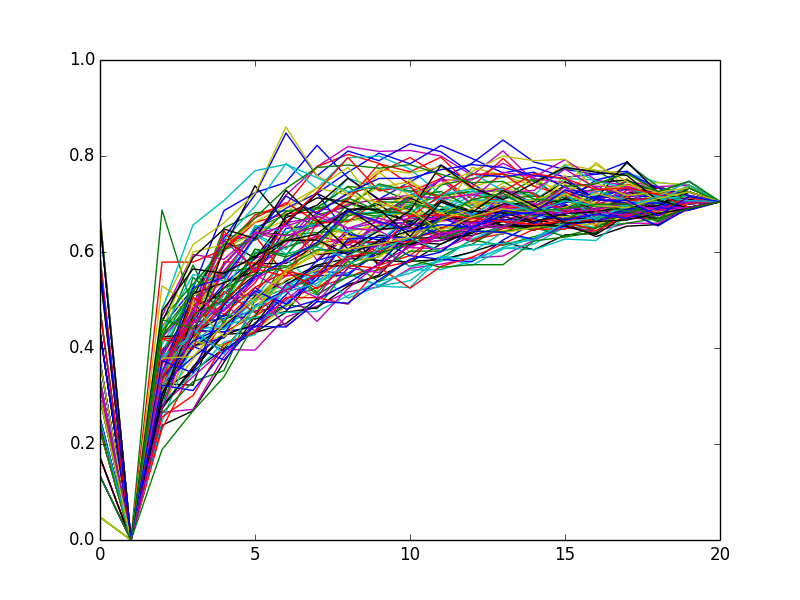
\includegraphics[width=2.0in, height=1.5in] {majority_p(edge=1|obs=1)_advice_shuffles.png}
		\caption{A subfigure}\label{fig:1a}
	\end{subfigure}
	%%%%%%%%      If you just have blank lines, it chokes. With COMMENTS, it's fine.
	\begin{subfigure}[b]{.3\linewidth}
		\centering
		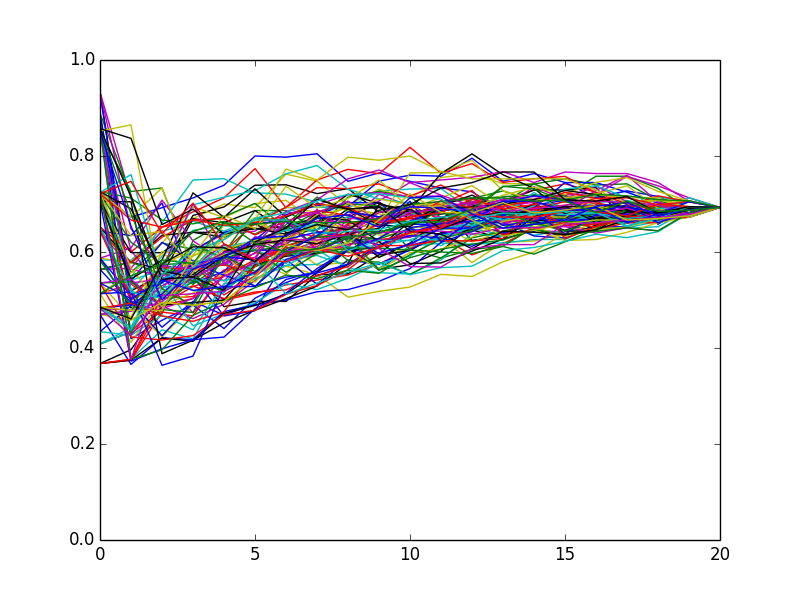
\includegraphics[width=2.0in, height=1.5in]{neighbor_p(edge=1|obs=1)_advice_shuffles.png}
		\caption{Another subfigure}\label{fig:1b}
	\end{subfigure}
	%%%%%%%%     And I just wasted a way to break the code up visually.	
	\begin{subfigure}[b]{.3\linewidth}
		\centering
		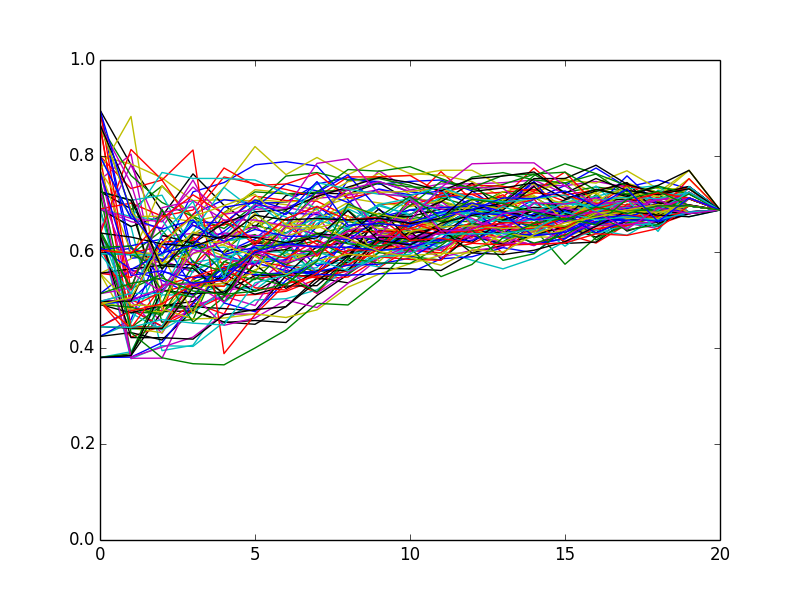
\includegraphics[width=2.0in, height=1.5in]     {block_p(edge=1|obs=1)_advice_shuffles.png}
		\caption{Another subfigure}\label{fig:1c}
	\end{subfigure}
	\caption{FIRST Row}
	%%%%%%%%%%%%%%%%%%%%%%%%%%%%%
	\begin{subfigure}[b]{.3\linewidth}
		\centering
		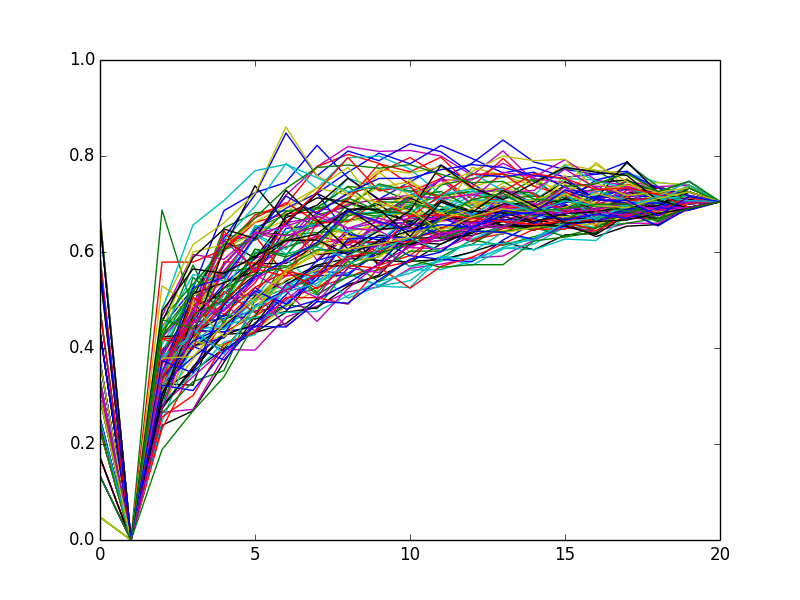
\includegraphics[width=2.0in, height=1.5in] {majority_p(edge=1|obs=1)_advice_shuffles.png}
		\caption{A subfigure}\label{fig:1a}
	\end{subfigure}
	%%%%%%%%
	\begin{subfigure}[b]{.3\linewidth}
		\centering
		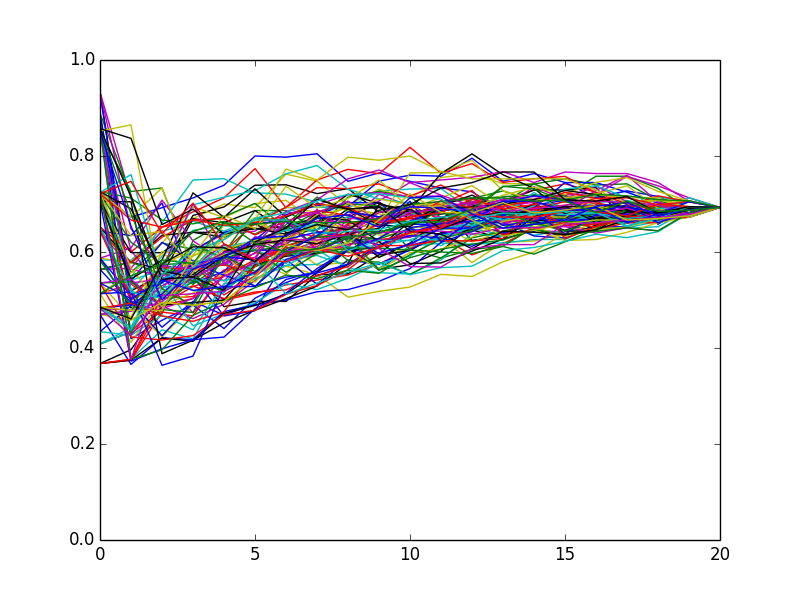
\includegraphics[width=2.0in, height=1.5in]{neighbor_p(edge=1|obs=1)_advice_shuffles.png}
		\caption{Another subfigure}\label{fig:1b}
	\end{subfigure}
	%%%%%%%%   
	\begin{subfigure}[b]{.3\linewidth}
		\centering
		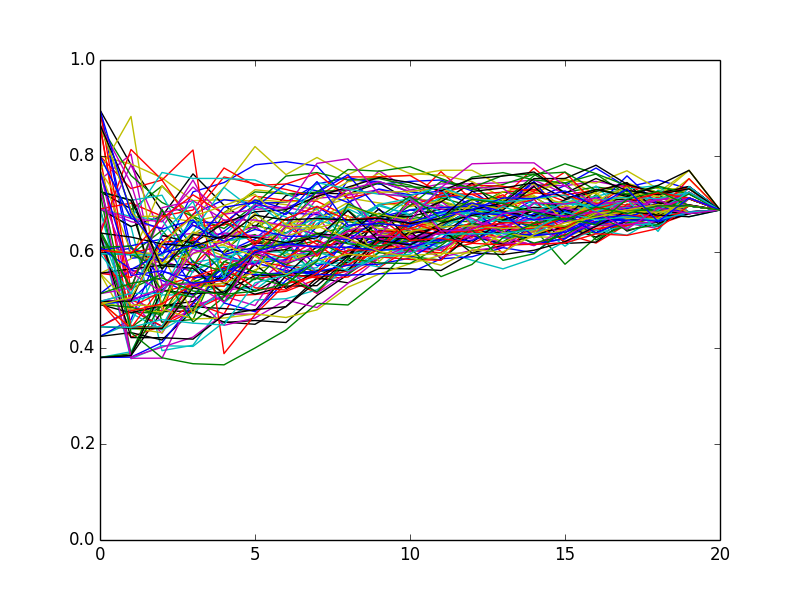
\includegraphics[width=2.0in, height=1.5in]     {block_p(edge=1|obs=1)_advice_shuffles.png}
		\caption{Another subfigure}\label{fig:1c}
	\end{subfigure}
	\caption{SECOND Row}
	
\end{figure}

%
%\begin{figure}[!ht]
%\centering
%
%\subfloat[Majority  ]{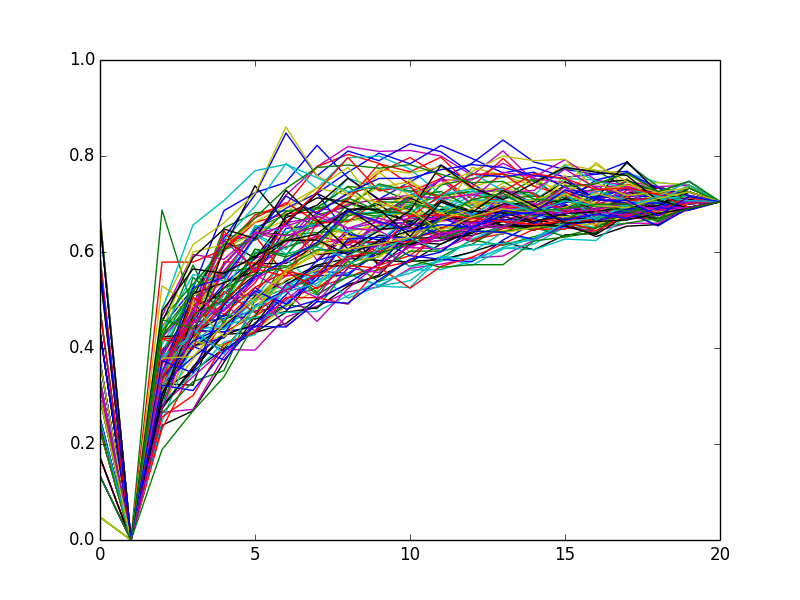
\includegraphics[width=2.0in, height=1.5in] {majority_p(edge=1|obs=1)_advice_shuffles.png}}
%\subfloat[Neighbor]{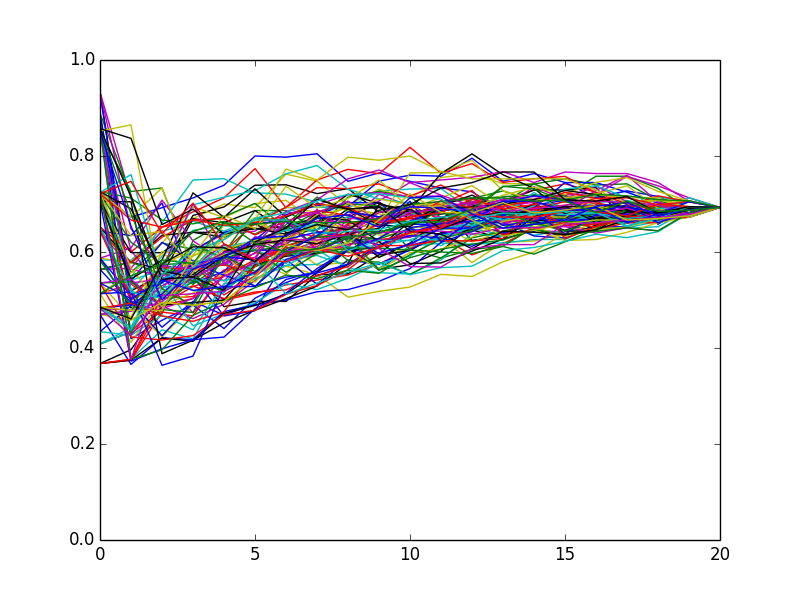
\includegraphics[width=2.0in, height=1.5in]{neighbor_p(edge=1|obs=1)_advice_shuffles.png}}
%\subfloat[Block      ]{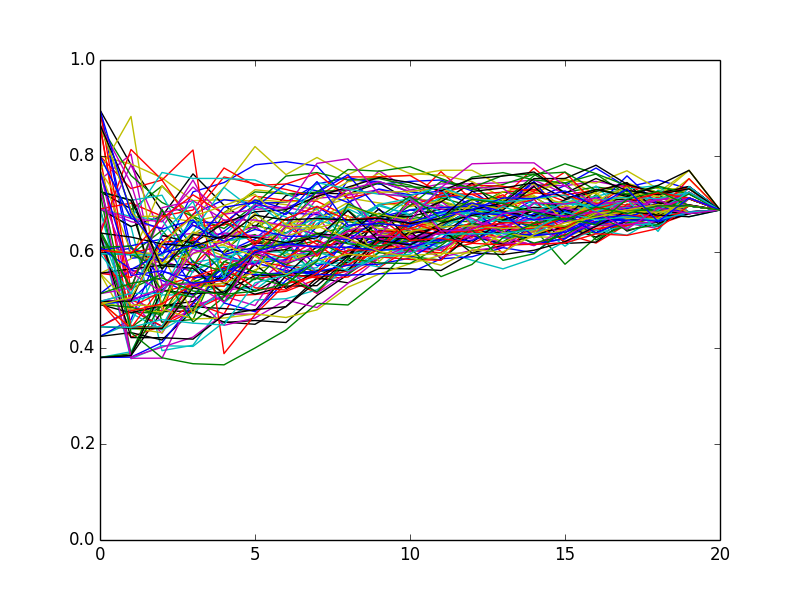
\includegraphics[width=2.0in, height=1.5in]     {block_p(edge=1|obs=1)_advice_shuffles.png}}
%\\
%\subfloat[Majority  ]{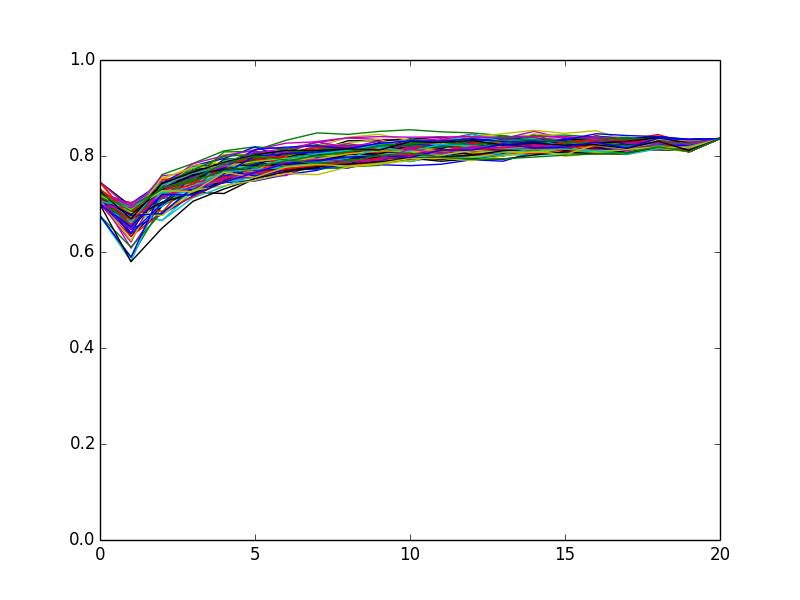
\includegraphics[width=2.0in, height=1.5in] {majority_p(edge=0|obs=0)_advice_shuffles.png}}
%\subfloat[Neighbor]{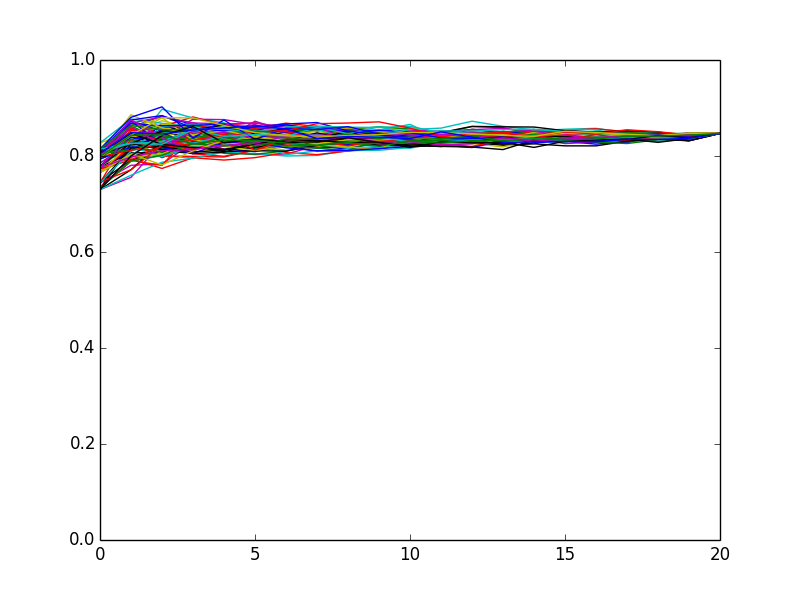
\includegraphics[width=2.0in, height=1.5in]{neighbor_p(edge=0|obs=0)_advice_shuffles.png}}
%\subfloat[Block      ]{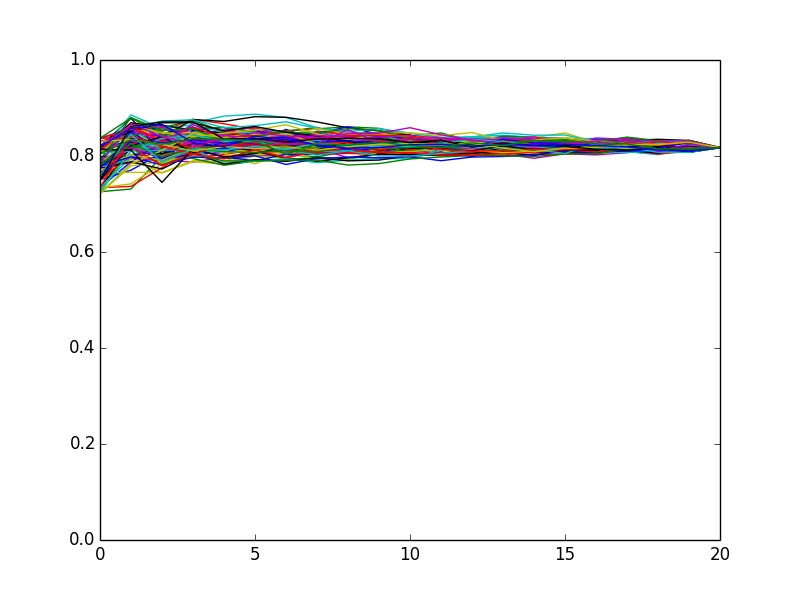
\includegraphics[width=2.0in, height=1.5in]     {block_p(edge=0|obs=0)_advice_shuffles.png}}
%\\
%\subfloat[Majority  ]{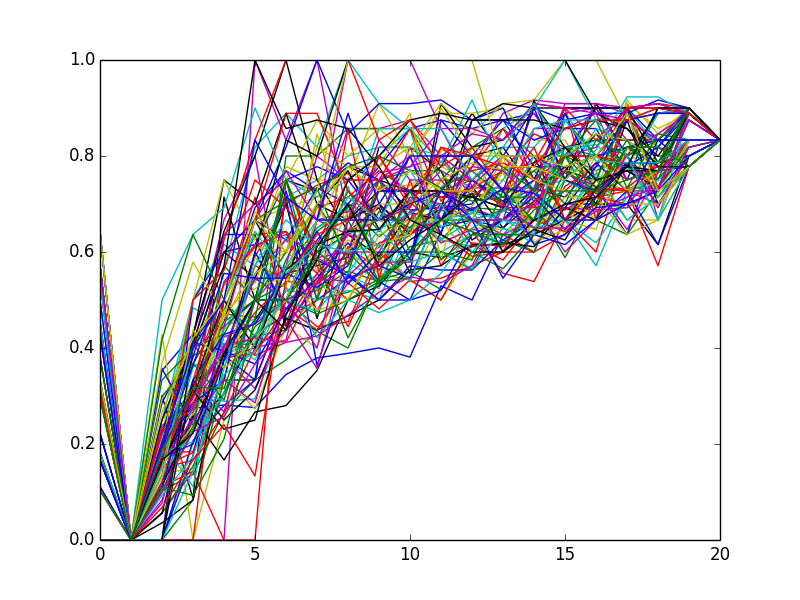
\includegraphics[width=2.0in, height=1.5in] {majority_p(edge=1|obs=1)_friendship_shuffles.png}}
%\subfloat[Neighbor]{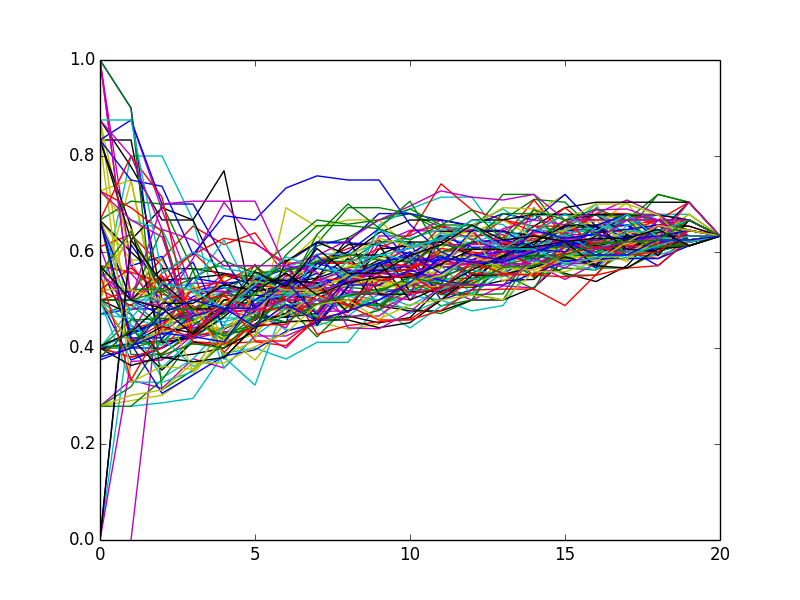
\includegraphics[width=2.0in, height=1.5in]{neighbor_p(edge=1|obs=1)_friendship_shuffles.png}}
%\subfloat[Block      ]{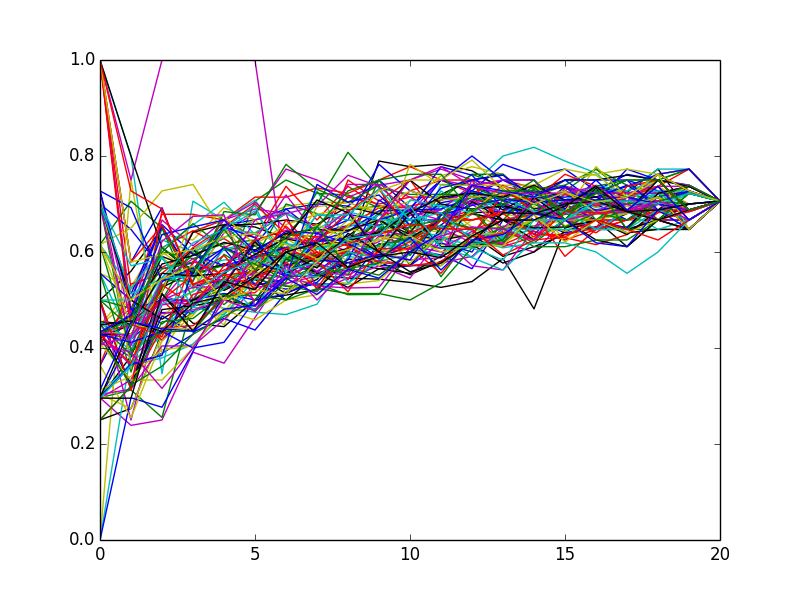
\includegraphics[width=2.0in, height=1.5in]     {block_p(edge=1|obs=1)_friendship_shuffles.png}}
%\\
%\subfloat[Majority  ]{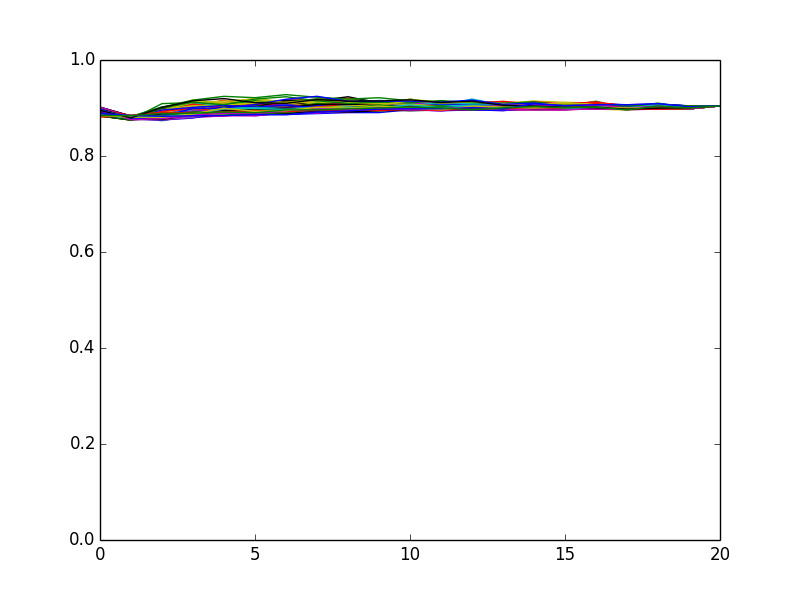
\includegraphics[width=2.0in, height=1.5in] {majority_p(edge=0|obs=0)_friendship_shuffles.png}}
%\subfloat[Neighbor]{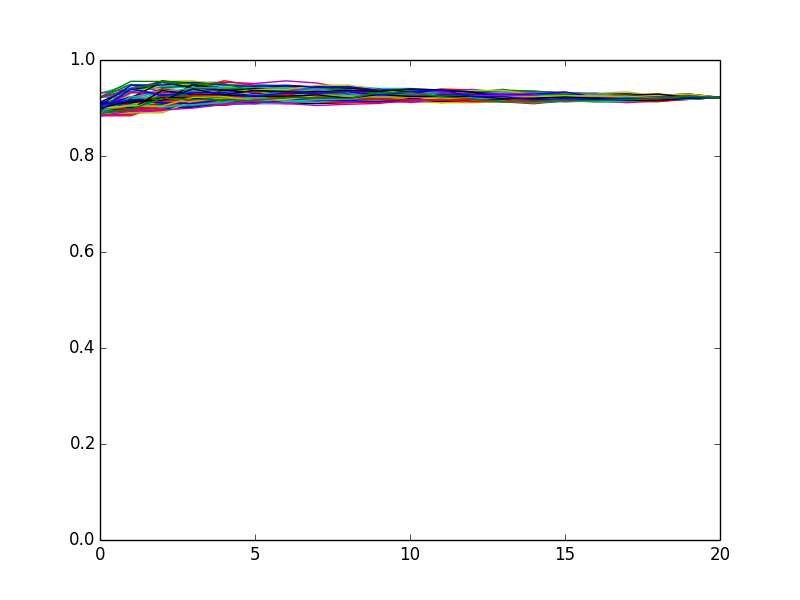
\includegraphics[width=2.0in, height=1.5in]{neighbor_p(edge=0|obs=0)_friendship_shuffles.png}}
%\subfloat[Block      ]{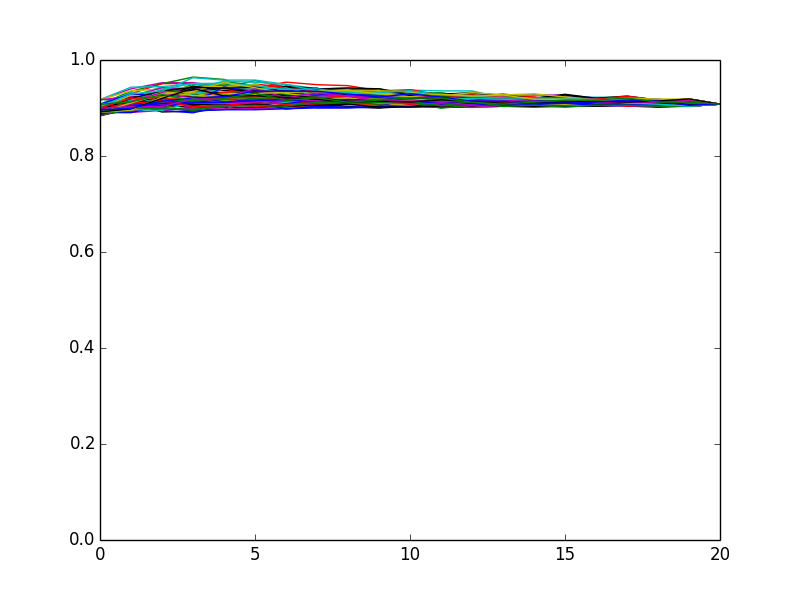
\includegraphics[width=2.0in, height=1.5in]     {block_p(edge=0|obs=0)_friendship_shuffles.png}}
%
%\caption{P(edge $\mid$ obs) Using Different Voting Rules}
%\label{fig:edge_given_obs}
%\end{figure} 
%
%\begin{figure}[!ht]
%\centering
%
%\subfloat[Majority  ]{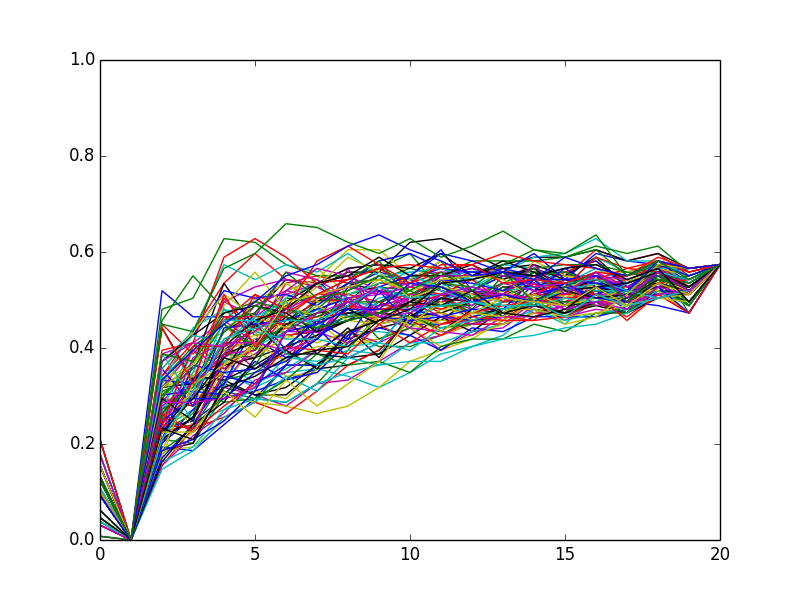
\includegraphics[width=2.0in, height=1.5in] {majority_p(obs=1|edge=1)_advice_shuffles.png}}
%\subfloat[Neighbor]{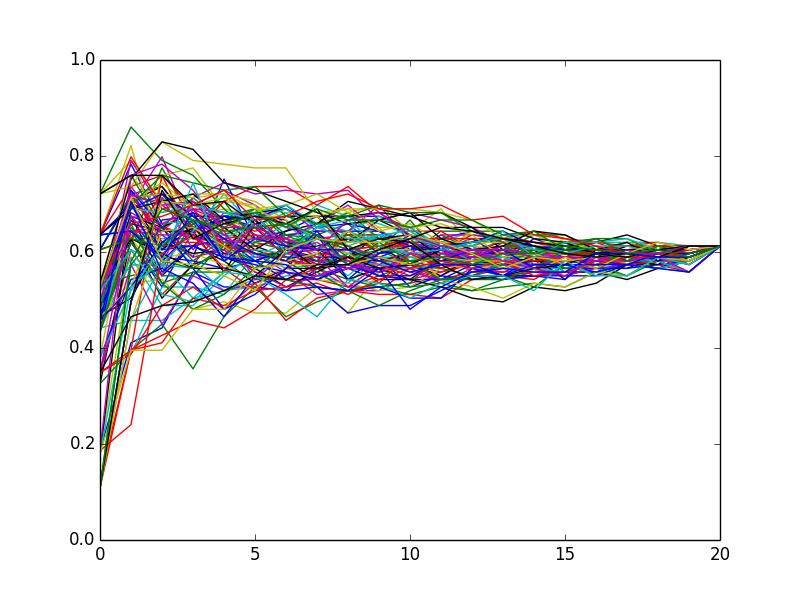
\includegraphics[width=2.0in, height=1.5in]{neighbor_p(obs=1|edge=1)_advice_shuffles.png}}
%\subfloat[Block      ]{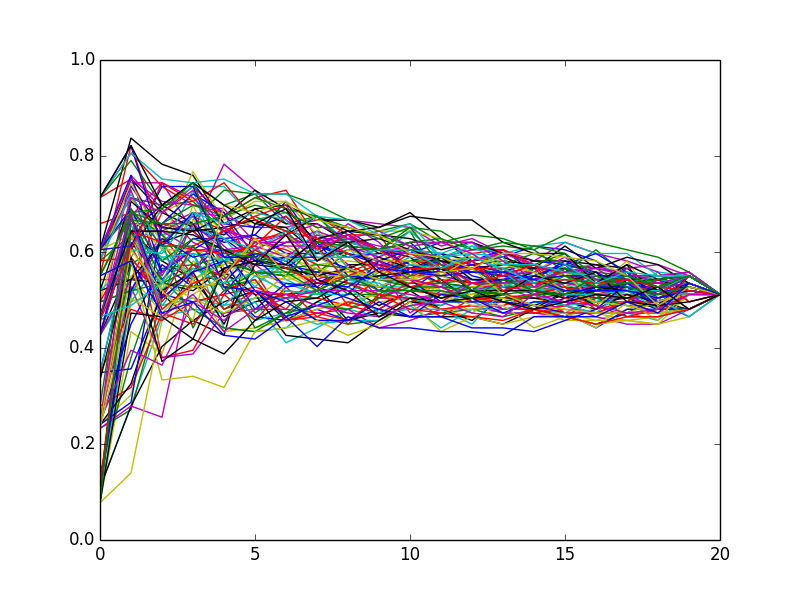
\includegraphics[width=2.0in, height=1.5in]     {block_p(obs=1|edge=1)_advice_shuffles.png}}
%\\
%\subfloat[Majority  ]{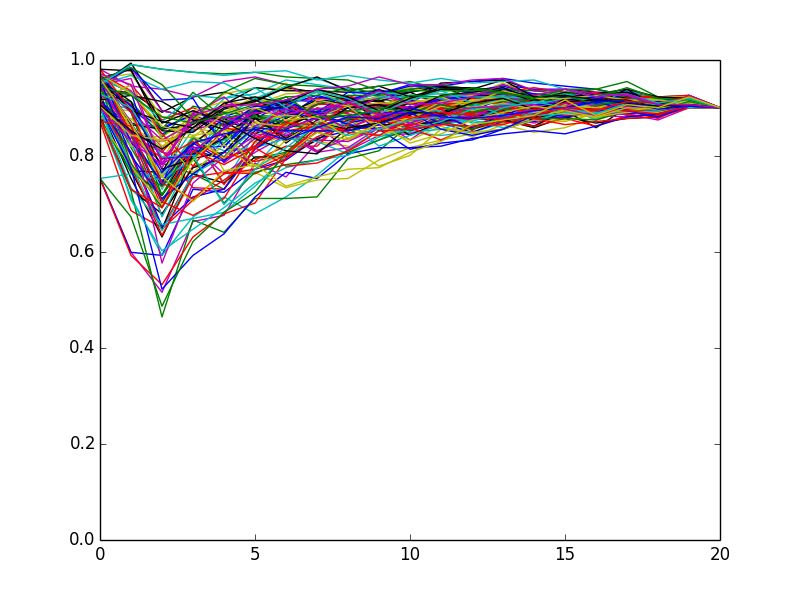
\includegraphics[width=2.0in, height=1.5in] {majority_p(obs=0|edge=0)_advice_shuffles.png}}
%\subfloat[Neighbor]{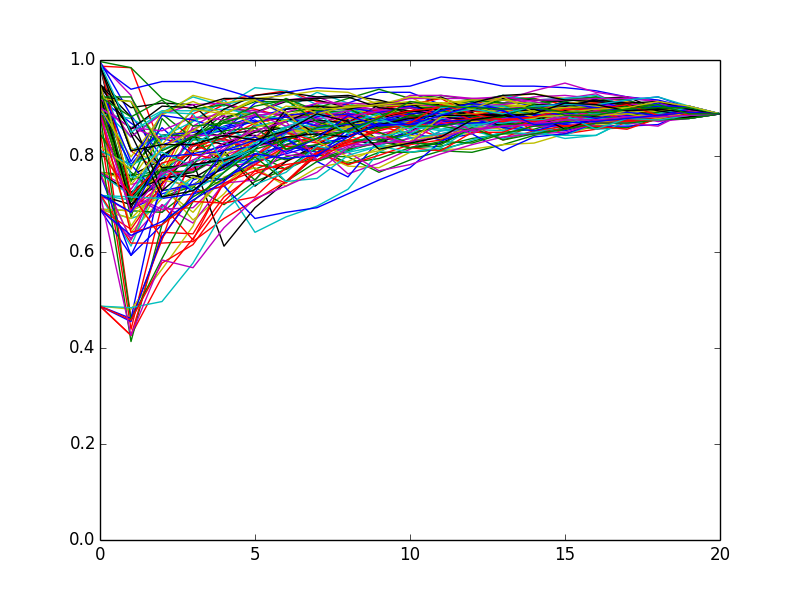
\includegraphics[width=2.0in, height=1.5in]{neighbor_p(obs=0|edge=0)_advice_shuffles.png}}
%\subfloat[Block      ]{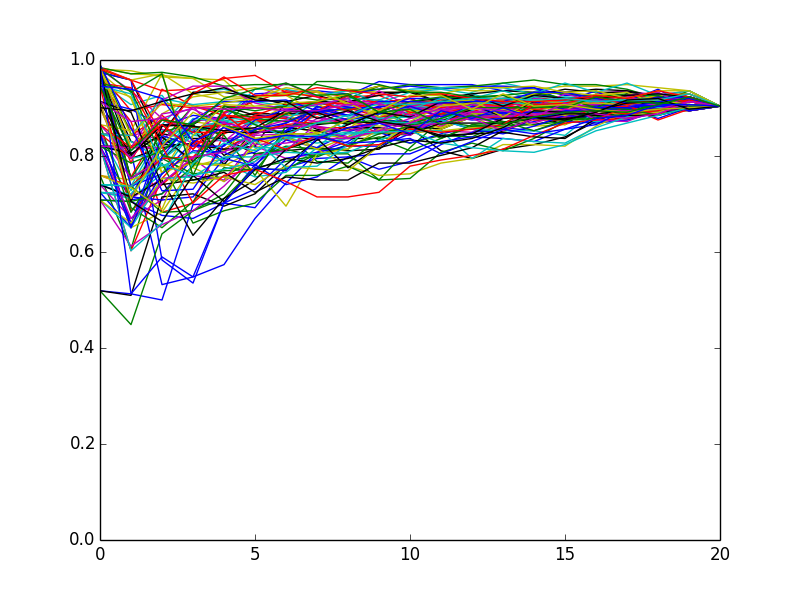
\includegraphics[width=2.0in, height=1.5in]     {block_p(obs=0|edge=0)_advice_shuffles.png}}
%\\
%\subfloat[Majority  ]{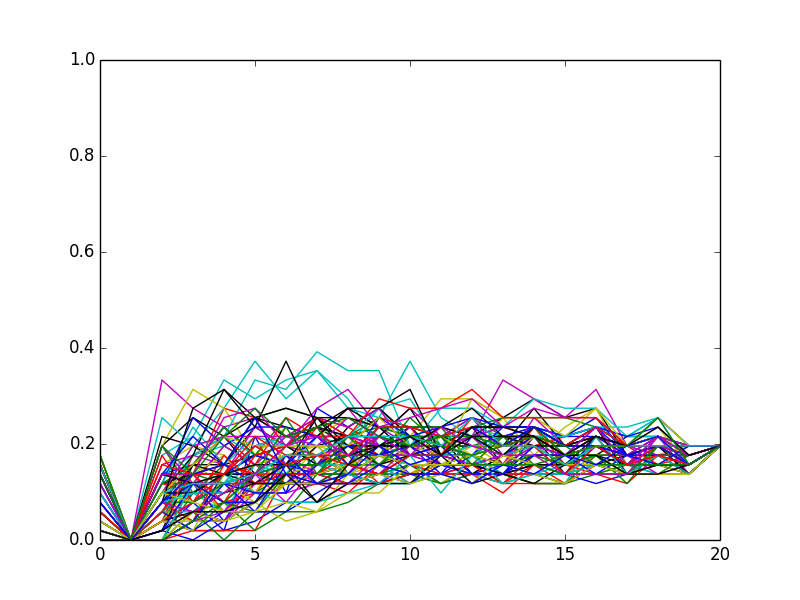
\includegraphics[width=2.0in, height=1.5in] {majority_p(obs=1|edge=1)_friendship_shuffles.png}}
%\subfloat[Neighbor]{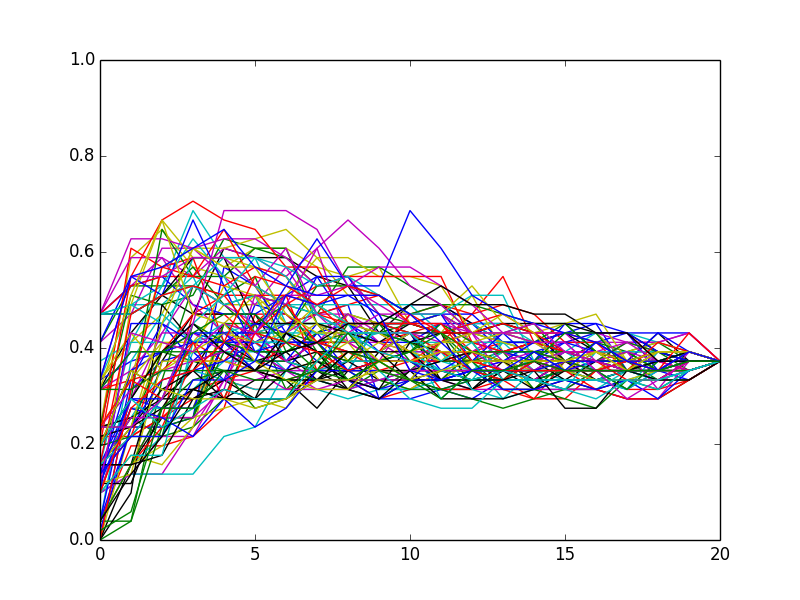
\includegraphics[width=2.0in, height=1.5in]{neighbor_p(obs=1|edge=1)_friendship_shuffles.png}}
%\subfloat[Block      ]{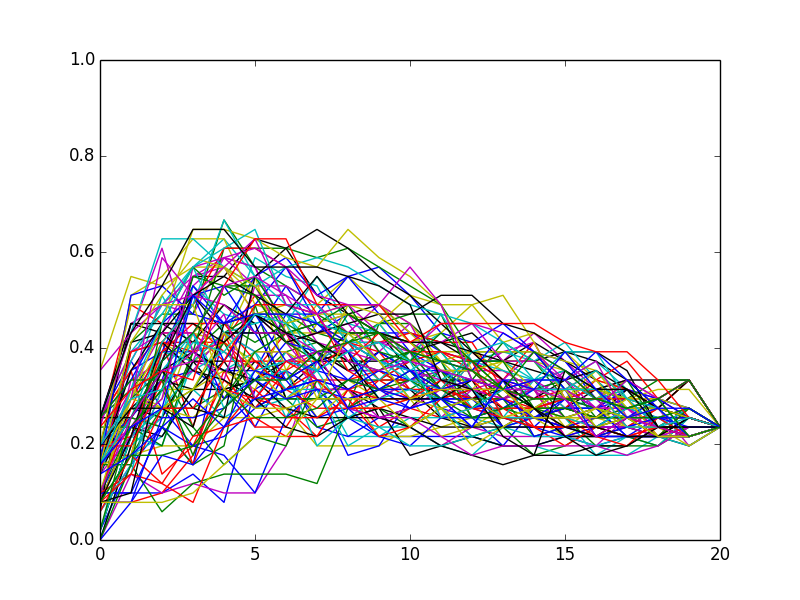
\includegraphics[width=2.0in, height=1.5in]     {block_p(obs=1|edge=1)_friendship_shuffles.png}}
%\\
%\subfloat[Majority  ]{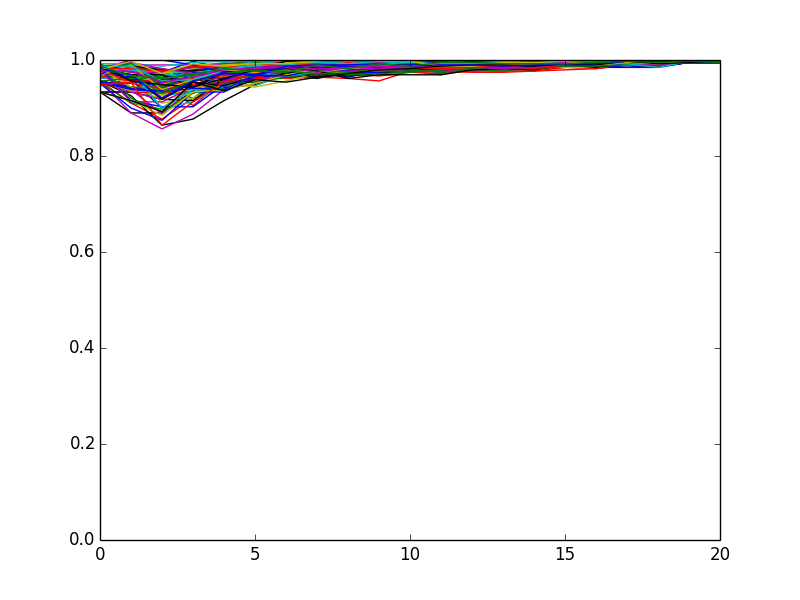
\includegraphics[width=2.0in, height=1.5in] {majority_p(obs=0|edge=0)_friendship_shuffles.png}}
%\subfloat[Neighbor]{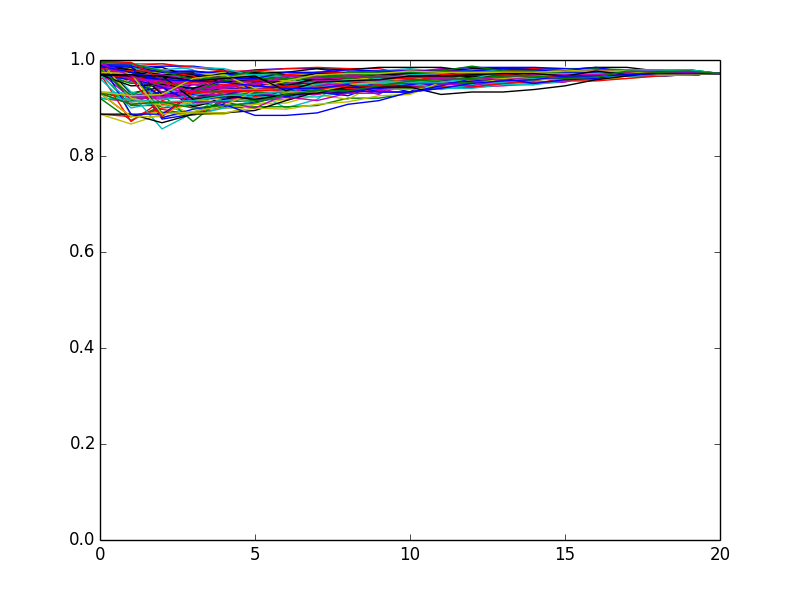
\includegraphics[width=2.0in, height=1.5in]{neighbor_p(obs=0|edge=0)_friendship_shuffles.png}}
%\subfloat[Block      ]{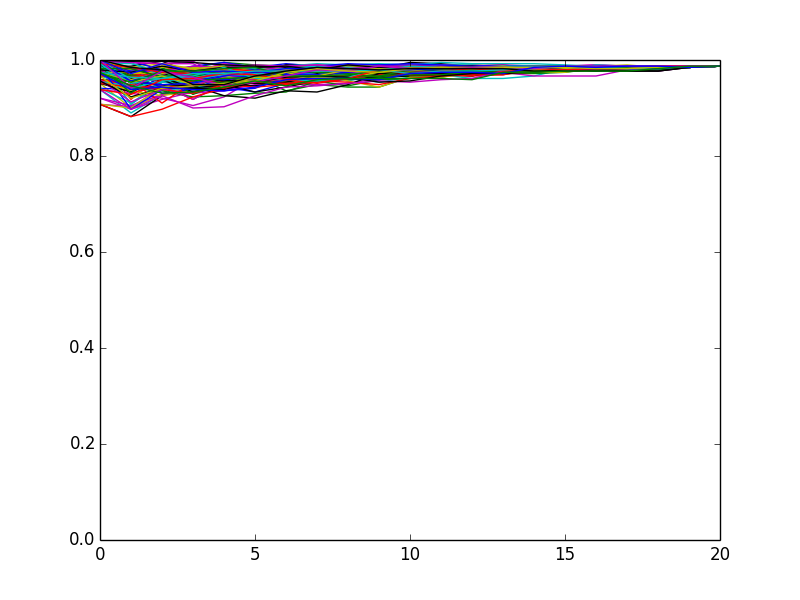
\includegraphics[width=2.0in, height=1.5in]     {block_p(obs=0|edge=0)_friendship_shuffles.png}}
%
%\caption{P(obs $\mid$ edge) Using Different Voting Rules} % AND USING DIFFERENT NUMBERS OF PEOPLE
%\label{fig:obs_given_edge}
%\end{figure} 
%
%
%
%\begin{figure}[!ht]
%\centering
%
%\subfloat[Majority  ]{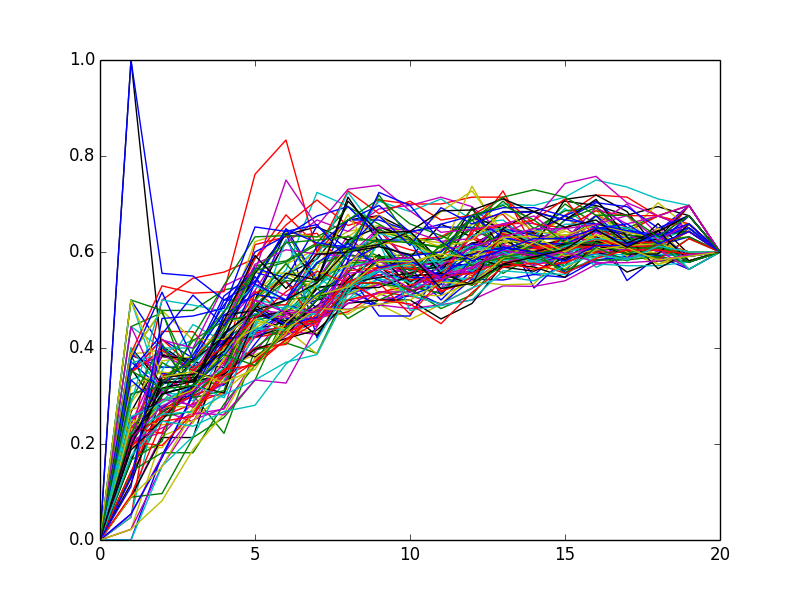
\includegraphics[width=2.0in, height=1.5in] {majority_p(edge=1|obs=1)_friendship_threshold=3.png}}
%\subfloat[Neighbor]{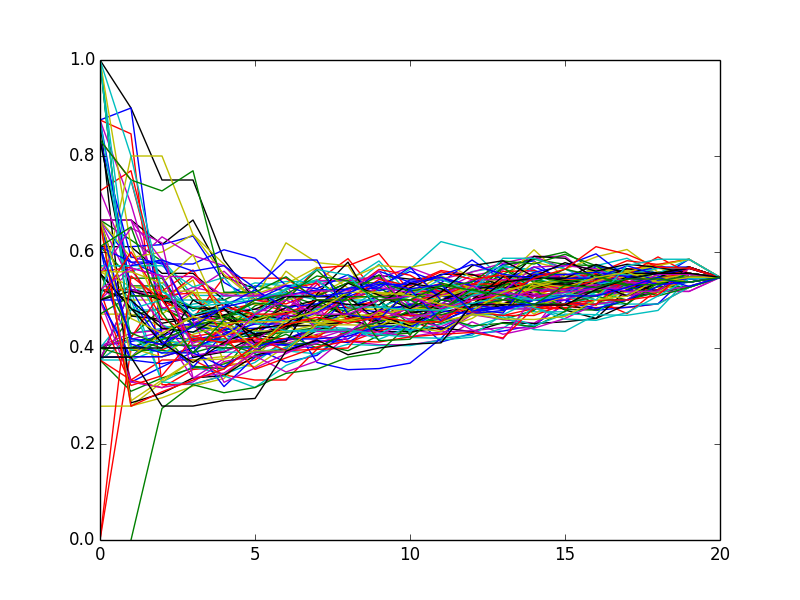
\includegraphics[width=2.0in, height=1.5in]{neighbor_p(edge=1|obs=1)_friendship_threshold=3.png}}
%\subfloat[Block      ]{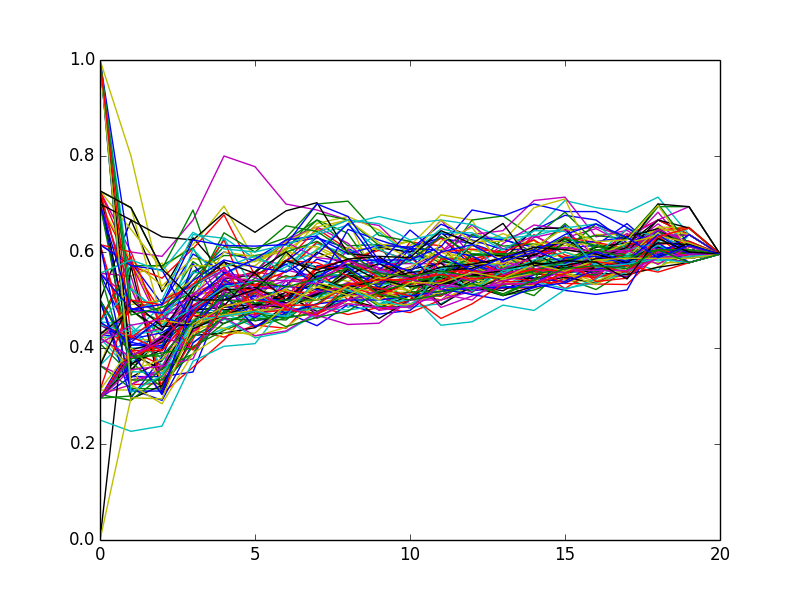
\includegraphics[width=2.0in, height=1.5in]     {block_p(edge=1|obs=1)_friendship_threshold=3.png}}
%\\
%\subfloat[Majority  ]{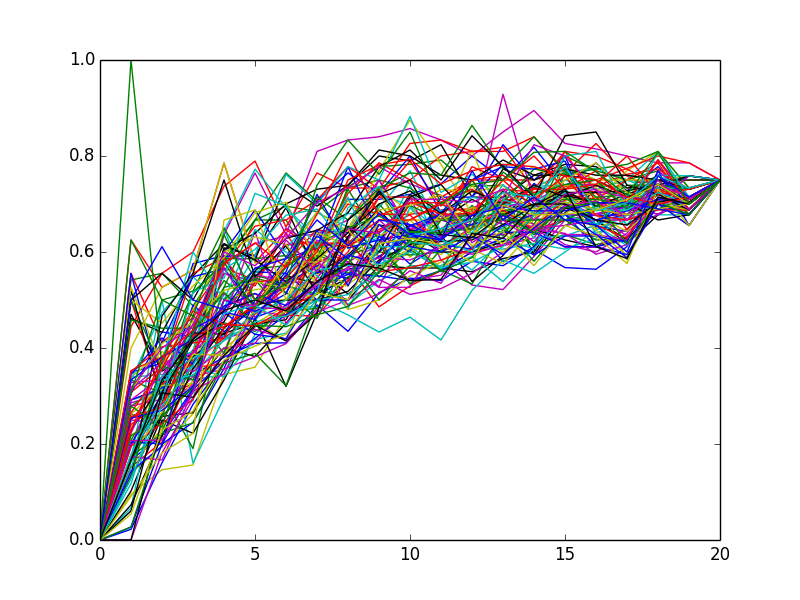
\includegraphics[width=2.0in, height=1.5in] {majority_p(edge=1|obs=1)_friendship_threshold=4.png}}
%\subfloat[Neighbor]{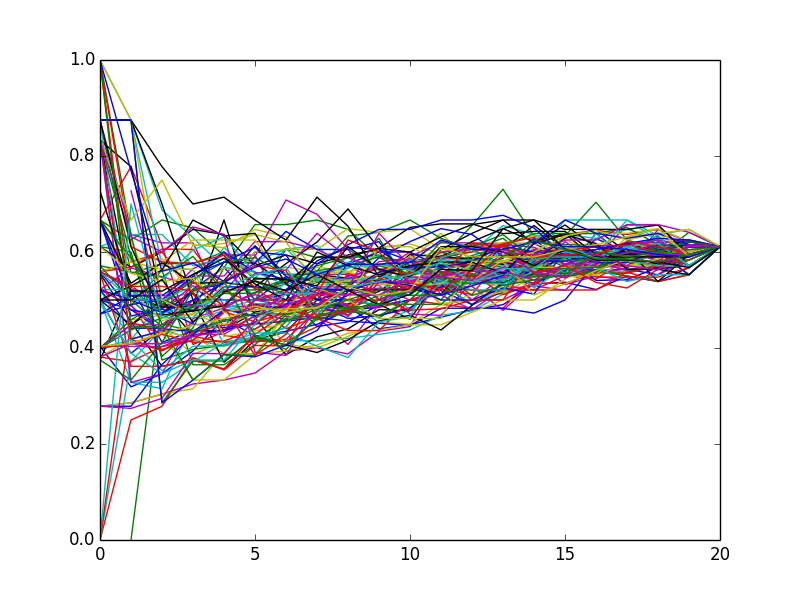
\includegraphics[width=2.0in, height=1.5in]{neighbor_p(edge=1|obs=1)_friendship_threshold=4.png}}
%\subfloat[Block      ]{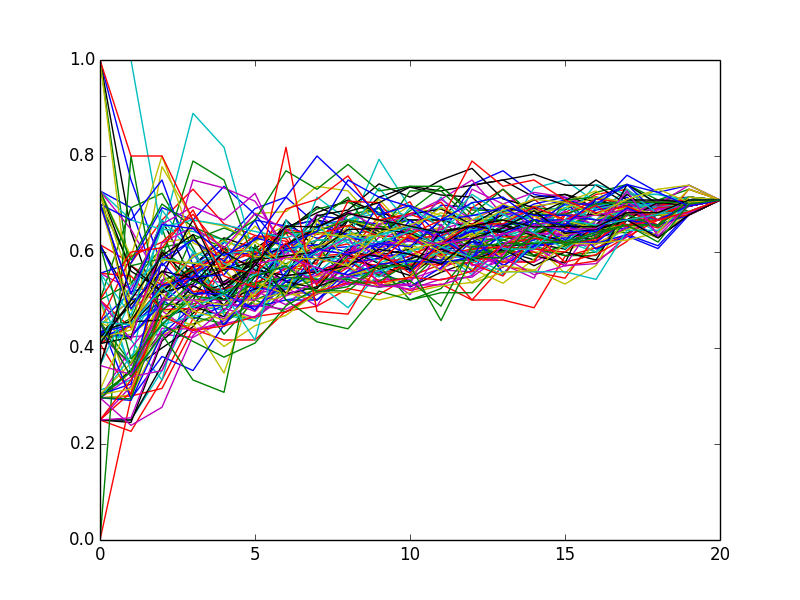
\includegraphics[width=2.0in, height=1.5in]     {block_p(edge=1|obs=1)_friendship_threshold=4.png}}
%\\
%\subfloat[Majority  ]{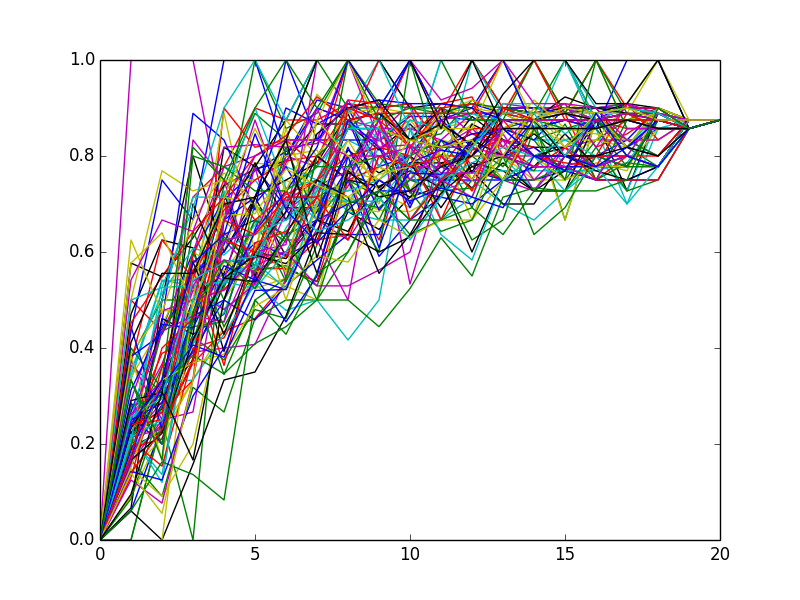
\includegraphics[width=2.0in, height=1.5in] {majority_p(edge=1|obs=1)_friendship_threshold=6.png}}
%\subfloat[Neighbor]{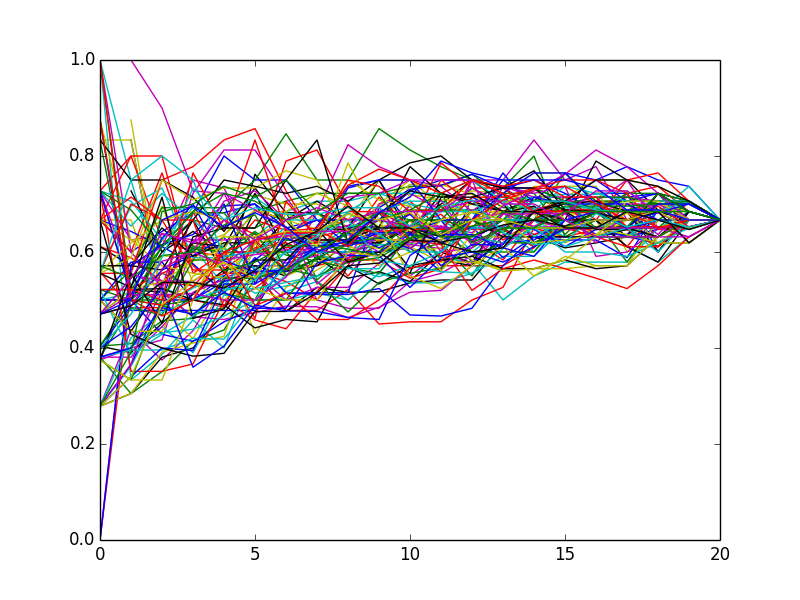
\includegraphics[width=2.0in, height=1.5in]{neighbor_p(edge=1|obs=1)_friendship_threshold=6.png}}
%\subfloat[Block      ]{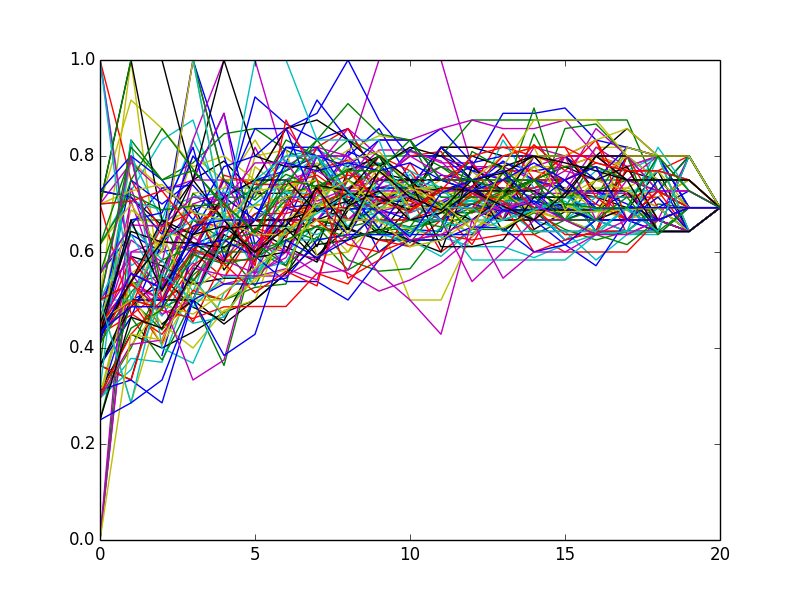
\includegraphics[width=2.0in, height=1.5in]     {block_p(edge=1|obs=1)_friendship_threshold=6.png}}
%\\
%\subfloat[Majority  ]{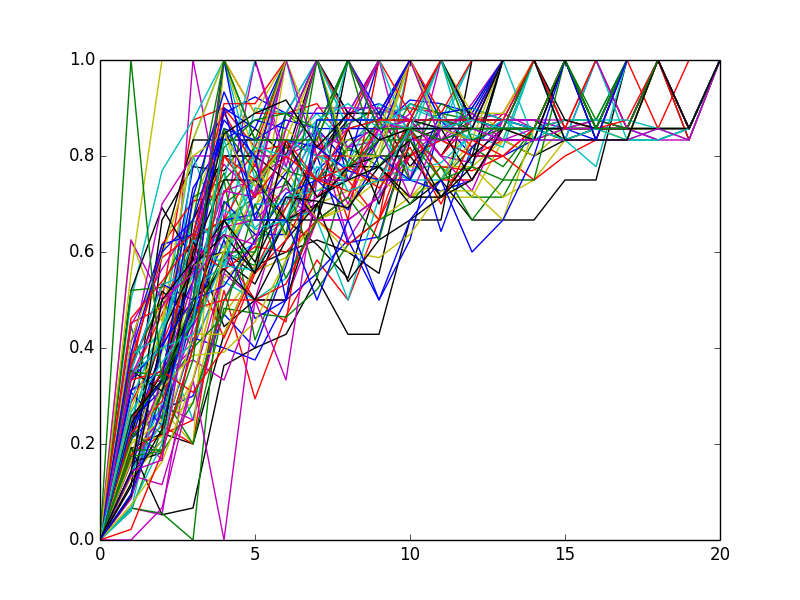
\includegraphics[width=2.0in, height=1.5in] {majority_p(edge=1|obs=1)_friendship_threshold=7.png}}
%\subfloat[Neighbor]{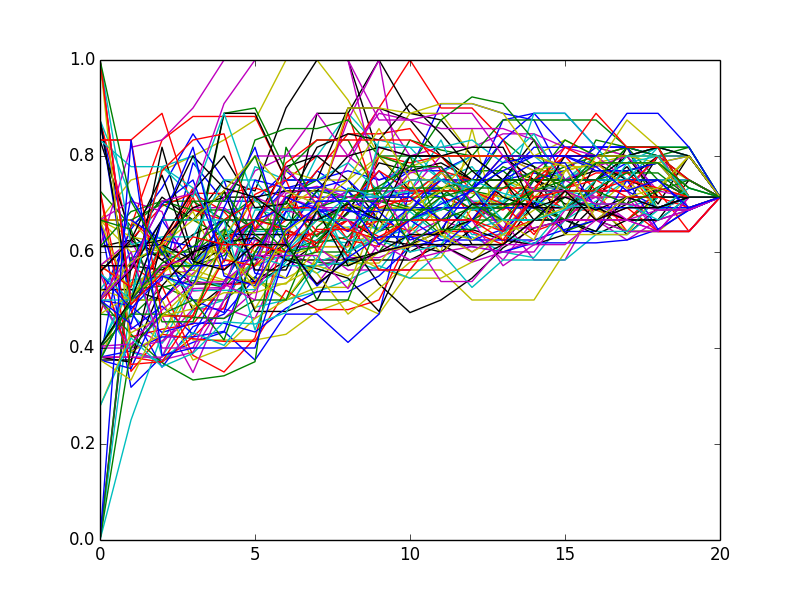
\includegraphics[width=2.0in, height=1.5in]{neighbor_p(edge=1|obs=1)_friendship_threshold=7.png}}
%\subfloat[Block      ]{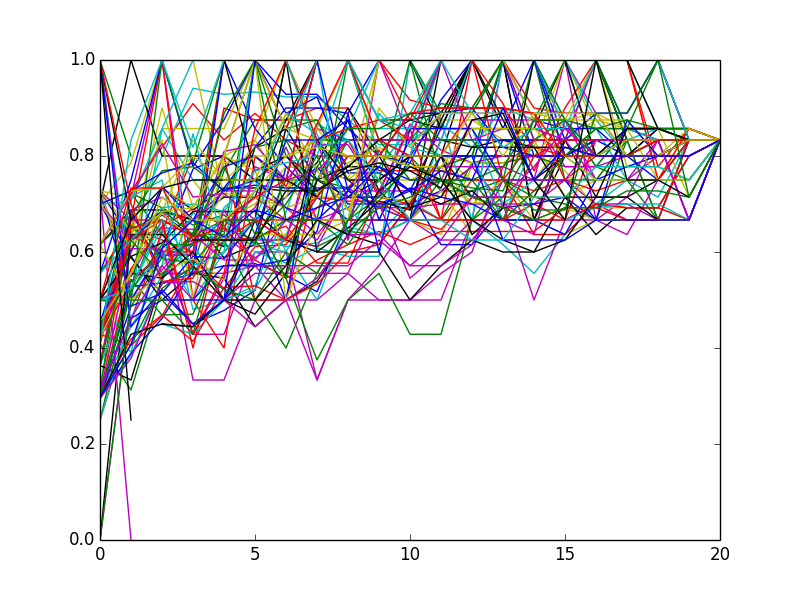
\includegraphics[width=2.0in, height=1.5in]     {block_p(edge=1|obs=1)_friendship_threshold=7.png}}
%
%\caption{P(edge $\mid$ ons) on Friendship Using Different Thresholds} % AND USING DIFFERENT NUMBERS OF PEOPLE
%\label{fig:thresholds}
%\end{figure} 


% Block Models of the consensus networks
%\begin{figure}[!ht]
%\centering
%\subfloat[Metropolis]{\label{fig:metropolis}\includegraphics[width=2.0in, height=1.5in]{first_fitting_graph_proud.png}}
%\subfloat[Gibbs]{\label{fig:gibbs}\includegraphics[width=2.0in, height=1.5in]{actual_gibbs_curve.png}}
%\caption{Likelihoods of Parameter Vectors During the Fitting Process}
%\label{fig:boxplots}
%\end{figure} 
%
%
%\begin{algorithm}
%\caption{The Metropolis Method}
%\begin{algorithmic}
%\For{$i = 1$ to num-iterations}
%\State $j \leftarrow \Call{randomchoice}{1:K}$
%\State $\theta_{new, j} \gets \theta_{j} + \Call{randomchoice}{[-1, 1]}$ \Comment{As long as it remains in bounds}
%\State $\theta_{new} \gets \Call{applyconstraint}{\theta, j}$ \Comment{Make $\theta$ non-decreasing, holding $\theta_j$ constant}
%\If{$\Call{min}{1, \frac{\ell(\theta_{new})}{\ell(\theta)}} > \Call{randomuniform}{[0,1)}$}
%\State $\theta \gets \theta_{new}$
%\If{\Call{likelihood}{$\theta$} $>$ \Call{likelihood}{$\theta_{max}$}}
%\State $\theta_{max} \gets \theta$
%\EndIf
%\EndIf
%\EndFor
%\State \Call{return}{$	\theta_{max}$}
%\end{algorithmic}
%\end{algorithm}

\end{document}  